\section{Is everything sunshine, if I simply want it?}

\begin{center}
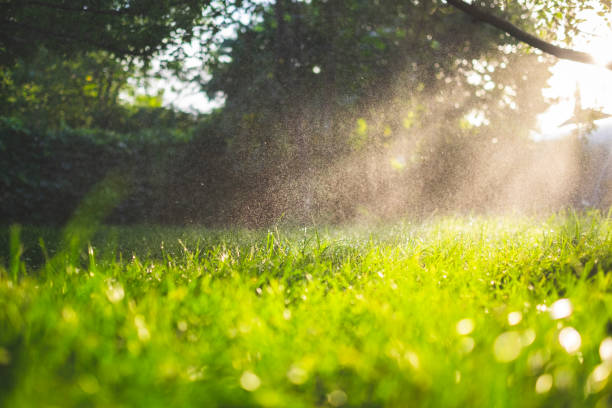
\includegraphics[width=5cm]{images/20_sunshine.jpg}
\end{center}

Whoever believes that sunshine can be created by simply visualising it is naive, or has let themselves be convinced by toxic positive-thinkers. Sunshine can't be wished from existence. Sunshine either is, or it isn't. Right...?!

When my child is sick, or my husband feels attracted to another woman, when my neighbour plays Heavy Metal at two o'clock in the morning, or when I'm in sheer panic of going to that meeting tomorrow at work, it is of little value to convince myself that everything is completely different than it is. Also physical pain, let's say sciatica, can only be made to disappear (through meditation, breathing) by only very few.

Common people like us rely on being somehow able to deal gracefully with the lack of sunshine in one way or the other. That's not easy, but it's possible. An important tool is to be able to learn to love the rain.

"Great", you say, "I shall rejoice, even though my child has the measles and I have absolutely no clue what I should say at tomorrow's meeting?!" No, you do not necessarily have to do this with rejoice. Only... let's say, reduce the resistance a bit, so that there is some space to breathe. Because resistance is fear, and fear tightens you up, and when it gets tight, breathing is more difficult... and when we can't breathe properly, we neither can think straight nor feel sensitively.

Even the most sophisticated form of resistance will change absolutely nothing about the current facts, but simply use up all your energy until exhaustion. So just have a little bit less of it, ok? Good! Now we can finally breathe properly again. Aaaah. Rain is good for the environment. Measles is good for...? Ok, here is a list: Measles is good for staying at home with the little ones. For developing a deeper connection between us, while I swipe away the hair out of their faces. For reading to them from a book, which has been overdue for a long time. For the inspiration from this story for tomorrow's meeting (dragons can be friendly, too!). For those breathtaking 10 minutes of silence when she finally falls asleep. For this crazy (German: "ver-rückt", which literally means “shifted”) feeling of calmness in the eye of the tornado. Is this sunshine? Most probably not.

But it's a good, rich rain. One which washes away so much which has been dusty for so long. One to which you gladly turn your face and smile. If I can't have the sunshine, then I want to love the rain.
